\documentclass[a4paper, 12pt]{article}

\usepackage{hyperref}
\usepackage{fullpage}
\usepackage[top=0.5in, bottom=1.5in, left=0.5in, right=0.5in, footskip=4em]{geometry}
\usepackage{amsmath}
\usepackage{fancyhdr}
\usepackage[usenames,dvipsnames]{xcolor}
\usepackage{pgfornament}

\usepackage[shortlabels]{enumitem}
\usepackage{xspace}
\usepackage{lastpage}
\usepackage{multicol}
\usepackage{blindtext}
\usepackage{titling}
\usepackage{standalone}
\usepackage{amsfonts}
\usepackage[framemethod=TikZ]{mdframed}
\usetikzlibrary{calc}
\usepackage{lineno}
\usepackage{amsthm}
\usepackage{amssymb}
\usepackage{mathtools}
\usepackage{datetime}
\usepackage[most]{tcolorbox}
\usepackage{cancel}
\usetikzlibrary{tikzmark}
\linenumbers


%BEGIN_FOLD Commands
\newcommand{\half}{\frac{1}{2}}
\newcommand{\epv}[1]{\ensuremath{\left< #1 \right>}\xspace}
\newcommand{\variance}{\ensuremath{\text{Var}}}
\newcommand{\eout}{\ensuremath{E_\text{out}}\xspace}
\newcommand{\ein}{\ensuremath{E_\text{in}}\xspace}
\newcommand{\cx}{\ensuremath{\mathcal{X}}\xspace}
\newcommand{\cz}{\ensuremath{\mathcal{Z}}\xspace}
\newcommand{\real}{\mathbb{R}}
\DeclareSymbolFont{extraup}{U}{zavm}{m}{n}
\DeclareMathSymbol{\varheart}{\mathalpha}{extraup}{86}
\DeclareMathSymbol{\vardiamond}{\mathalpha}{extraup}{87}
\renewcommand{\heartsuit}{\textcolor{red}{\varheart}}
\renewcommand{\diamondsuit}{\textcolor{red}{\vardiamond}}
\newcommand{\definition}{\noindent\textbf{Def:} }
\newcommand{\theorem}{\noindent\textbf{Theorem:} }
\newcommand{\predicate}{\noindent\textbf{Inductive Predicate:} }
\newcommand{\inductivestep}{\noindent\textbf{Inductive Step:} }
\renewcommand{\proof}{\noindent\textbf{Proof:} }
\newcommand{\lemma}[1]{\noindent\textbf{Lemma #1:} }
\newcommand{\hint}{\textbf{Hint:} }
\newcommand{\basecase}{\noindent\textbf{Base Case:} }
\newcommand{\inductivehypothesis}{\noindent\textbf{Inductive Hypothesis:} }
\newcommand{\collorary}{\noindent\textbf{Collorary:} }
\newcommand{\qedd}{\qed\newline}
\newcommand{\kwd}[1]{\textcolor{blue}{\textbf{\underline{#1}}}}
\newcommand\ColorBox[2][]{%
	\stepcounter{mybox}%
	\node[draw=red!70!black,fill=red!20,align=left,#1] (box\themybox) {#2};
}
\newcommand{\expl}[2]{%
	\underset{\substack{\uparrow\\\mathrlap{\text{\hspace{-1em}#2}}}}{#1}}
\newcommand{\uexpl}[2]{%
	\overset{\substack{\mathrlap{\text{\hspace{-1em}#2}}\\\downarrow}}{#1}}
\newcommand{\st}{\text{ such that }}
%\newcommand{\qed}{\ensuremath{\blacksquare}}
%END_FOLD
\newcommand{\sidenote}[1]{\textcolor{gray}{#1}}

%BEGIN_FOLD miscellaneious default
\makeatletter
% Make a copy of macros responsible for entering display math mode
\let\start@align@nopar\start@align
\let\start@gather@nopar\start@gather
\let\start@multline@nopar\start@multline
% Add the "empty line" command to the macros
\long\def\start@align{\par\start@align@nopar}
\long\def\start@gather{\par\start@gather@nopar}
\long\def\start@multline{\par\start@multline@nopar}
\makeatother
\setlength{\columnsep}{1cm}
%opening
\setlength{\abovedisplayskip}{-\baselineskip}%
\setlength{\abovedisplayshortskip}{\abovedisplayskip}%

\pagestyle{fancy}
\renewcommand{\headrulewidth}{0pt}
\lfoot{\small{\course}: Week \weekno}
\rfoot{\small{\thetitle}}
\rhead{}
\cfoot{\pgfornament[height=1em, ydelta=-0.4em]{17} \thepage of \pageref{LastPage}  \pgfornament[height=1em, ydelta=-0.4em]{18}}

\DeclareMathOperator{\sign}{sign}
\newcommand{\vect}[1]{\ensuremath{\mathbf{#1}}\xspace}

\tikzstyle{every picture}+=[remember picture]
\newcommand{\bwgrid}[1]{
	\def \aaa #1
	
	\foreach \y in {0,1,2} {
		\foreach \x in {0,1,2} {
			\pgfmathsetmacro{\clr}{\aaa[\x][\y]}
			%\message{aaa \clr}
			\definecolor{MyColor}{rgb}{\clr,\clr,\clr}
			\path[fill=MyColor] (\x,\y) rectangle ++(1,1); 
		}
	}
	\draw[step=1cm,very thin] (0,0) grid (3,3);	
}

\setenumerate{label=\alph*.)}
\definecolor{db}{RGB}{100,65,23}
\newtheoremstyle{examplestyle}% name
{}%         Space above, empty = `usual value'
{}%         Space below
{}% Body font
{}%         Indent amount (empty = no indent, \parindent = para indent)
{}% Thm head font
{}%        Punctuation after thm head
{\newline}% Space after thm head: \newline = linebreak
{\textbf{\textcolor{db}{\thmname{#1}\thmnumber{ #2}:} \thmnote{ #3}}}%         Thm head spec
\theoremstyle{examplestyle}

\newtheorem{examplethm}{Example}
\newenvironment{example}[1][]{\begin{mdframed}[style=example]\begin{examplethm}[#1]}{\end{examplethm}\end{mdframed}}

\newenvironment{example*}[1][]{\begin{mdframed}[style=example]\begin{examplethm}[#1]\end{examplethm}}{\end{mdframed}}
\newenvironment{Figure}
{\par\medskip\noindent\minipage{\linewidth}}
{\endminipage\par\medskip}
\newenvironment{formula}{
	\begin{mdframed}[style=formula]
	}{
\end{mdframed}}
%END_FOLD

\newcommand{\course}{Discrete Math}
\title{Induction}
\newcommand{\weekno}{2}

\begin{document}
\begin{center}
	\textcolor{orange}{\textsc{\course}}\\
	\huge\textbf{\textsc{\thetitle}}\\
	\small\textcolor{gray}{Last updated:\, \today \, \currenttime}\\
	\pgfornament[width=0.7\textwidth, color=white!30!black]{88}
\end{center}

\begin{multicols}{2}
	Imagine we are trying to construct a long line of dominoes and you plan to make it falls one after another. We want to make the whole things falls. There are two things that you need to make sure that you did two things.
	\begin{enumerate}		
			\item We need to push the first dominoes. 
			\begin{center}
				$d_1$ falls.
			\end{center}
		\item First, we need to make sure that you place them close enough such that when one dominoes fall then the next one will fall. Specificall
		\begin{center}
			If $d_n$ falls, then $d_{n+1}$ will too falls.
		\end{center}

	\end{enumerate}
	
	Of course, we need to place them close enough. But if we only place them close enough but we did not push the first dominoes, then the dominoes will just stand there. On the other hand, if we push the first dominoes but we place them so far away from each other that when one falls it doens't even touch the next one then not all dominoes will fall. You need them both.
	
	Now let use the same idea for our proof technique. Suppose we want to prove that some predicate $P(n)$ is \emph{true} for all $n \ge 1$. We can use the dominoes idea. We need to show that
	\begin{enumerate}
		\item $P(1)$ is true.
		\item If $P(k)$ is true for some $k$, then the next one $P(k+1)$ has to be true.
		
		Concretely, for $k=6$, we want to show that if $P(6)$ is true then that will also make $P(7)$ true. We show it for any general $k\ge 1$.
	\end{enumerate} 
	
\section*{Weak Induction}

Let us look at the first example of how to use induction to prove some theorem.

\theorem $\forall n \in I$, $n\ge 1$
\[
	1+2+3+ \ldots + n = \frac{n(n+1)}{2}.
\]

\proof 

Let us first defined exactly what is the predicate $P$ that is our domino pieces.
\newline

\predicate
\[
	P(s) := 1 + 2 + 3 + \ldots +s = \frac{s(s+1)}{2}
\]
It should be emphasized that \underline{$P$ is NOT a number}. $P$ is a predicate. It is a function that returns true or false. For our case, $P$ is a function that checks when you plug in number for $s$ whether the sum of 1 to $s$ is equal to $\frac{s(s+1)}{2}$ or not. If it does eqaul then it returns true. If it does not equal then it returns false. For example, $P(2)$ checks whether $1+2=3$ equals to $\frac{2(3)}{2} = 3$ or not. Since, they are equal, $P(2)$ is true.
\newline

\basecase Here we want to make sure that the first dominoes falls. The base case is usally simple. So, here we want to check if $P(1)$ is true. To do that we just plug it in.
\[
	1 = \frac{1(1+1)}{2}\;\checkmark
\]
 So, $P(1)$ is true and we are done with the base case. Yes, it is that simple.
 \newline
 
\inductivestep In the inductive step, we want to make sure that the dominoes are close enough. So the thing we want to show is that if $P(k)$ is true for some $k$ then $P(k+1)$ is also true. So let us write that out what exactly do we mean by $P(k)$ is true and what exactly do we want to show.

First, we assume that $P(k)$ is true \emph{for some} integer $k$. That means
\[
	1 + 2 + 3 + \ldots + k = \frac{k(k+1)}{2}
\]
We call this the \kwd{inductive hypothesis}(IH).

It is important to note that for this inductive hypothesis. We only assume that LHS and RHS\footnote{Left hand side and Right hand side} are equal for a particular fixed number $k$. We \emph{do not} assume it for all $k$. We just need it for one particular value of $k$.

Now, the thing we want to show is that $P(k+1)$ is also true. That means we want to show(WTS) that
\begin{align}
1 + 2 + 3 + \ldots + k + (k+1) &= \frac{(k+1)((k+1)+1)}{2}\\
&=\frac{(k+1)(k+2)}{2}
\label{eq:wts1}
\end{align}

\proof We want to show the above proposition given the inductive hypothesis. Let us first consider the left hand side of \ref{eq:wts1}.
\[
	LHS = 1 + 2 + 3 + \ldots + k + (k+1)	
\]

From our inductive hypothesis we know that
\[
	1 + 2 + 3 + \ldots + k = \frac{k(k+1)}{2}	
\]

Therefore,
\begin{align*}
	LHS &= \underbrace{1 + 2 + 3 + \ldots + k}_{\text{From our IH}} + (k+1)\\
	& = \underbrace{\frac{k(k+1)}{2}}_{{\text{From our IH}}} + (k+1) \\
	& = (k+1)\left(\frac{k}{2}+1\right)\\
	& = \frac{(k+1)(k+2)}{2}
\end{align*}

Which is exactly the right handside of the thing we are trying to prove
\[
RHS = \frac{(k+1)(k+2)}{2}
\]

Therefore,
\begin{align*}
1 + 2 + 3 + \ldots + k + (k+1) &= \frac{(k+1)(k+2)}{2}\\
LHS &= RHS
\end{align*}

So we are done with the inductive step. \qed

Therefore, by mathematical induction,
\[
1+2+3+ \ldots + n = \frac{n(n+1)}{2} \; \forall n \in I, n\ge1
\]
\qedd

Let us consider another example:

\theorem$\forall n \in I, n \ge 1$
\[
1+3+5+7+\ldots+(2n-1) = n^2 
\]

\proof We are going to do this by mathematical induction
\newline
\predicate
\[
P(s) := 1+3+5+7+\ldots+(2s-1) = s^2
\]

\basecase $P(1)$
\[
1 = 1^2 \checkmark
\]

\inductivestep Let us assume that $\exists k \ge 1$
\[
1+3+5+7+\ldots+(2k-1) = k^2 
\]
We want to show that
\begin{align*}
1+3+\ldots+(2k-1) + (2(k+1) -1 ) &= (k+1)^2  \\
1+3+\ldots+(2k-1) + (2k + 1) &= (k+1)^2 
\end{align*}

The left hand side of the WTS is
\begin{align*}
LHS &= \underbrace{1+3+\ldots+(2k-1)}_{\text{IH}} + (2k + 1)\\
&= \underbrace{k^2}_{\text{IH}} + 2k + 1\\
&= (k+1)^2\\
&= RHS
\end{align*}

Therefore by mathematical induction $\forall n \in I, n \ge 1$
\[
1+3+5+7+\ldots+(2n-1) = n^2 
\]
\qedd

For the above theorem, it is much better to do geometric proof you can google for one. This is the cons of mathematical induction. It tells you that it works but most of the time it does not tell you why it works.

Let us consider the next example.

\theorem If $n \in \mathbb{O}$ and $n\ge1$ then $n^2 -1$ is a multiple of 4.

\proof We are going to prove this by mathematical induction.

\predicate First let us define our inductive predicate
\[
	P(s) := s^2 - 1 \text{ is a multiple of }4.
\]
\basecase $P(1)$
\[
	1 - 1 = 0 = 4 \times 0 \checkmark
\]
\inductivestep
Let us assume that $\exists k \ge 1$
\[
	k^2-1 = 4q
\]
for some integer $q$. We want to show that
\begin{align}
	(k+2)^2 -1 &= 4 r
	\label{eq:wts2}
\end{align}
for some integer $r$.

\sidenote{Notice that we use $k+2$ here instead of $k+1$ since we want to show this for all odd integers.}

Let us consider the LHS of \ref{eq:wts2}.
\begin{align*}
	(k+2)^2 -1 &= k^2 +4k +4 -1\\
	&= \underbrace{k^2 -1}_{4q\text{ by IH}} + 4k + 4
	&= 4q + 4k + 4\\
	& = 4(q + 4k + 1)\\
	& = 4r
\end{align*}
\qed

Therefore, by mathematical induction
\[
n^2 -1\text{ is a multiple of 4 }\forall n \in \mathbb{O}, n\ge1
\]
\qedd

Sometimes the induction doesn't even have to do with number. Let us consider a $2^n \times 2^n$ square grid. Suppose that we take out the middle piece. We want to know whether we can tile the entire grid with L-shape triminoes.
\begin{center}
	\includestandalone[width=\linewidth]{grid}
\end{center}

\theorem $2^n \times 2^n$ grid with center taken out can be tiled with L shape triminoes.

\basecase $n=1$. Yes, we can fill it. \checkmark.

\begin{center}
	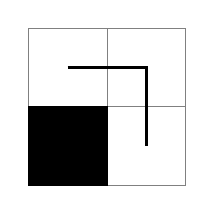
\begin{tikzpicture}%[show background grid]
		\draw[step=1cm,gray,very thin] (0,0) grid (2,2);
		\draw[fill=black](0,0) rectangle (1,1);
		\draw[very thick] (0.5, 1.5) -- (1.5, 1.5) -- (1.5,0.5);
	\end{tikzpicture}
\end{center}

\inductivestep
Let us assume that we can fill $2^k \times 2^k$ grid with the \kwd{center} taken out. Now we want to show that we can fill $2^{k+1} \times 2^{k+1}$ grid with the \kwd{center} piece taken out with L shape triminoes.

It is tempting to say that $2^{k+1} \times 2^{k+1}$ is just 4 of $2^k \times 2^k$ grids.

However, you can't get the missing center piece. But, in the mean while we realized that our life would be much easier if our assumption is that we can do it for $2^k \times 2^k$ \emph{any} piece missing then our job would be simple. Since we can put an L triminoes, at the center and we can use the inductive hypothesis as the figure below shown.

\begin{center}
	\includestandalone[width=0.8\linewidth]{grid2}
\end{center}

It is generally easier in induction to prove a stronger theorm since the hard part for induction prove is the inductive step and the easy part of if is the basecase. Changing the theorem to a more general one make the base case a bit harder but it will make the inductive step much easier since stronger theorem gives you a stronger inductive hypothesis. So, let us try to prove a stronger version of our previous theorem.

\theorem $2^n \times 2^n$ grid with one piece missing at \emph{any} place can be tiled with L-shaped triminoes.
\proof
\newline
\predicate $P(s):= 2^s \times 2^s$ grid with any piece missing can be filled with L-shaped triminoes.

\basecase $n=1$. Yes, we can fill it. But, this time we to show it for \emph{any} piece missing. So, there are actually 4 cases to consider but they are all symmetric.  \checkmark
\begin{center}
	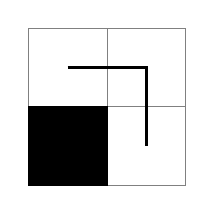
\begin{tikzpicture}%[show background grid]
	\draw[step=1cm,gray,very thin] (0,0) grid (2,2);
	\draw[fill=black](0,0) rectangle (1,1);
	\draw[very thick] (0.5, 1.5) -- (1.5, 1.5) -- (1.5,0.5);
	\end{tikzpicture}
\end{center}
\inductivestep
Let us assume that we can fill $2^k \times 2^k$ board with \emph{any} piece missing with L-shaped triminoes for some fixed $k$.

Now we want to show that we can fill $2^{k+1} \times 2^{k+1}$ with \emph{any} piece missing with L-shaped triminoes.

What we need to prove now is actually stronger that what we need last time but we have a stronger inductive hypothesis as well.

Let us consier a $2^{k+1} \times 2^{k+1}$ with \emph{any} piece missing. This piece must be in one of the quadrant.

\includestandalone[width=0.8\linewidth]{grid3}

We can then put L-shaped triminoes at the center like in the picture above. Then, each quadrant is a  \underline{$2^{k} \times 2^{k}$ with \emph{any} piece missing}.

Then we can use the inductive hypothesis on on each quadrant. That is by IH, we can fill each quadrant with L-shaped triminoes.

Therefore, we can fill $2^{k+1} \times 2^{k+1}$ grid with any piece missing with L-shaped triminoes.

Therefore by mathematical induction, we can fill any $2^n \times 2^n$ grid with any piece missing with L-shaped triminoes. \qedd

\collorary We can therefore fill in $2^k \times 2^k$ grid with the center piece missing.

\section*{Strong Induction}

In the previous section we have seen a type of mathematical induction called weak induction. In the induction step of weak induction, we require exactly 1 previous case to be true to make the next one true. 

If we think about the falling dominoes analogy. Once we get to the step where we need to push the sixth dominoes. We already have the 1st--5th dominoes fallen. In proving some theorem, we may need the combined power of the all the previous dominoes to make the next one fall.

Let us look at an example

\theorem Every integer greater than 1 is a product of primes.

\proof We will prove this by strong induction.

\predicate $P(s)$ := $s$ is a product of prime.

\basecase $P(2)$ 2 = 2 which is a product of prime.

\inductivestep

Let us assume that $P(i)$ is true $\forall i \ge k$. That is all the number less than or equal to $k$ is a product of prime.

Now we want to show that $P(k+1)$ is true. That is $k+1$ is a product of primes.

So we have to consider two cases:

First if $k+1$ is already a prime then we are done it is a product of primes by definition.

If $k+1$ is not a prime. That means there exists a prime $p$ that divides $k+1$. That is
\[
	k+1 = p q
\]

Since $q < k$, we can use inductive hypothesis that $q$ is a product of primes.

Therefore, since $k+1 = pq$, $k+1$ is a product of primes. 

Thus, by mathematical induction every integer greater than 1 is a product of primes.\qedd

From the above example you can see that we assume that all the previous number is a product of prime since in the induction proving step we didn't know where $q$ will end up but we know that $q$ ends up in some previous number for sure. We did not even care what is the prime factorization of $q$ all we care is that $q$ is a product of prime. This is an important idea for writing recursion function. You break the problem in to smaller problems. Then, you let it go by trusting that the same function can solve smaller problem.

Let us now consider splitting an $n\times m$ rectangular chocolate bar. Now we want to break it until they are all single $1\times 1$ blocks. If you count how many turns it takes. You will realized that it always takes $mn-1$ turns.
\begin{center}
	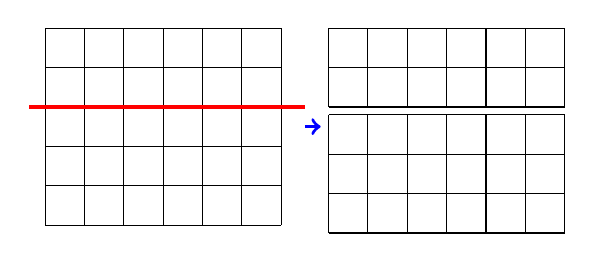
\begin{tikzpicture}
	\draw[step=0.5] (0,0) grid (3,2.5);
	\draw[red, very thick] (-0.2, 1.5) -- (3.3, 1.5);
	\draw[blue, ->, very thick] (3.3,1.25) -- (3.5,1.25);
	\begin{scope}
	\begin{scope}[yshift=1.5cm, xshift=3.6cm]
		\draw[step=0.5] (0,0) grid (3,1);
	\end{scope}
	\begin{scope}[yshift=-0.1cm, xshift=3.6cm]
	\draw[step=0.5] (0,0) grid (3,1.5);
	\end{scope}
	\end{scope}
	\end{tikzpicture}
\end{center}

Let us prove this fact

\theorem Breaking an $m\times n$ chocolate bar takes $mn-1$ turns.

This theorem is hard to prove since you have two variables to work with. It is much easier to induct on the number of pices. So let us rewrite the theorem.

\theorem Breaking an $n$ pieces rectangular chocolate bar takes $n-1$ turns.

\predicate $P(s):=$ breaking $s$ pieces rectangular chocolate bar takes $s-1$ turns.

\basecase $P(1)$. Of course if it is 1 by 1 chocolate piece we don't need to break it anymore. \checkmark

\inductivestep

Let us assume that $\forall i, 1 \ge i < k$ rectangular chocolate of size $i$ takes $i-1$ step to break into single pieces.

Now let us consider a chocolate of size $k$. We want to show that it will take $k-1$ turns to break it.

So, for chocolate of size $k$ if we do one break anywhere. We will end up with chocolate of size $p<k$ and $q<k$ such that $p+q=k$. Then all we need to do to break size $k$ chocolate is to break it once then break the other two pieces until they got to single pieces.

We know from our inductive hypothesis how many turns it takes to break the $p$ and $q$ chocolate since $p,q <$. Chocolate of size $p<k$ needs $p-1$ turns and chocolate of $q<k$ needs $q-1$ turns.

Therefore, the total number of turns needed is
\begin{align*}
	\text{turns} &= \expl{1}{$k \to p+q$} + \uexpl{(p -1)}{\text{break }p} + \expl{(q -1)}{\text{break }p}\\
	&=  p+q-1\\
	&= k-1
\end{align*}

So, we have proved that breaking $k$ pieces chocolate takes $k-1$ turns.

Therefore, by mathematical induction breaking $n$ pieces chocolate takes $n-1$ turns.\qedd

Let us consider the last example for strong induction. Let us consider a game where
\begin{enumerate}
	\item Each player starts with a stack of $n$ blocks.
	\item At each step player break one the available stacks into two stacks. $n \to p+q$
	\item The scored for the stack is computed by multiplying the number of block in the two stack the player just break. For example, if the player break a 5 block stack in to a stack of 3 and 2. Then the player get $3\times 2 = 6$ points.
	\item The two stack will then be avaiable to unstack. The game is then repeated from step 2 until all stacks are 1. 
\end{enumerate}

\theorem At the end of stacking game of $n$ block the player will get the score of $\frac{n(n-1)}{2}$

\proof We are going to prove this by induction

\predicate $P(s):=$ stacking game of $s$ blocks will give the score of $\frac{s(s-1)}{2}$.

\basecase $P(1)$ well you can't break it anymore so the score is 0=$\frac{1(1-2)}{2}$\checkmark.

\inductivestep

\inductivehypothesis Let assume that stacking game of $i$ blocks give $\frac{i(i-1)}{2}$ points forall integer $i$, $1< i < k$

We want to show that the stacking game of $k$ blocks give $\frac{k(k-1)}{2}$ points.

Let us play the stacking game of $k$ blocks. Without loss of generality, let the first break be $k \to a + b$.

The score the player would get for this step is $a \times b$ by the rule of the game.

Then the player will need to unstack $a$. Since we know that $1\le a < k$, unstacking $a$ until it reaches single blocks gives $\frac{a(a-1)}{2}$ points.

Also for the $b$ stack. Since we know that $1 \le b < k$, unstacking $b$ until it reaches single blocks gives $\frac{b(b-1)}{2}$ points.

Therefore the total score of unstacking the block is
\begin{align*}
	\text{score} &= \expl{ab}{First break} + \expl{\frac{a(a-1)}{2}}{Unstacking $a$} + \expl{\frac{b(b-1)}{2}}{Unstacking $b$}\\
	&= \half \left( 2ab + a^2 -a + b^2 - b\right)\\
	&= \half \left((a+b)^2 - (a+b)\right)\\
	&= \half (k^2 - k)\\
	&= \frac{k(k-1)}{2}
\end{align*}
which is exactly what we are trying to show.

Therefore, by mathematical induction unstacking $n$ blocks gives $n(n-1)/2$ points $\forall n \ge 1$

\section*{Caveat}

Let us consider the following Wrong Proof

\textcolor{red}{\cancel{\theorem}} All horses are of the same color. In other words, in every set of $n\ge 1$ horses, all horses belong to one color \checkmark.


\textcolor{red}{\cancel{\proof}} Proof by wrong induction.

\predicate $P(s) = $every set of $s$ horses are of the same color.

\basecase $P(1)$ set of 1 horse. Of course it has only one horse therefore all horses belong to one color.

\inductivestep

\inductivehypothesis Let us assume that every set of $k-1$ horses are of the same color. Now we want to show that every set of $k$ horses are of the same color.
\begin{enumerate}
\item Let us consider a generic set of $k$ horses
\[
A = \{h_1, h_2, h_3, \ldots, h_{k-1}, h_{k}\}
\]

\item Let us consider the $k-1$ horse subset of the above set.
\[
B = \{h_1, h_2, h_3, \ldots, h_{k-1}\}	
\]

\item Since $B$ is a set of $k-1$ horses, all the horses in $B$ are of the same color. Let us call the color $c$.

\item\label{bad} In particular $h_1$ and $h_2$ are of the same color $c$.

\item Now let us consider a different $k-1$ horses subset of $A$.
\[
C = \{h_2, h_3, \ldots, h_{k-1},h_{k}\}	
\]
\item Since $C$ is also a set of $k-1$ horses, all the horse in $C$ are of the same color.

\item Therefore, we $h_2$ and $h_k$ have the same color.
\item Furthermore, since $h_2$ and $h_1$ color, $h_2$, $h_1$ and $h_k$ have the same color $c$.
\item Therefore $h_1, h_2, \ldots h_k$ have the same color.
\item By mathematical induction, all set of $n$ horse are of the same color.
\end{enumerate}
\qedd

It is clear that not all horses are of the same color. But what is wrong with the proof?

To understand what's wrong with the proof, we need to go back to the falling dominoes. First, we need to make sure that the first piece falls and we did make sure about that in the first place.

We also need to make sure that all the other pieces are close enough. This is the part where the proof fail. The proof works just fine for going from $P(300) \to P(301)$. However, the proof breaks down when we try to apply it to $P(1) \to P(2)$. Look closely at step \ref{bad} and onward. The idea of the proof hinges on the fact that we can get the common element when we break down the set. When we consider breaking down set of two horses in to two of set of one horse. We do not have common element between the two.


\subsection*{Gilbreath Principle}

Coming soon.








\end{multicols}




\end{document}
